%!TEX root = ./thesis.tex
%****************************************************************
% preamble only for part II 
%****************************************************************
\renewcommand{\appendixname}{PAPER} % chapter name to PAPER

\titlecontents{chapter}% <chapter-type>
  [4.8em]% <left>
  {\vspace*{1em}\bfseries\normalsize}% <above-code>
  {\hspace*{-4.8em}Paper\ \thecontentslabel:\quad}% <numbered-entry-format>
  {}% <numberless-entry-format>
  {\normalsize\hfill\contentspage}% <filler-page-format>

\fancyhf{}   % define header/footer layout
\fancyhead{} % get rid of the headers on plain pages
\renewcommand{\headrulewidth}{0pt} % and the line
% title font for paper titles  
\renewcommand{\chaptitlefont}{\bfseries\Large}

%****************************************************************
% Paper I
%****************************************************************

\chapter{Scientific Paper I}

\noindent List of authors\\

\noindent \textit{In \Proc \IntlConf \ldots} \textbf{LNCS}, 035303 (2017)
\cleardoublepage

% include paper pdf file
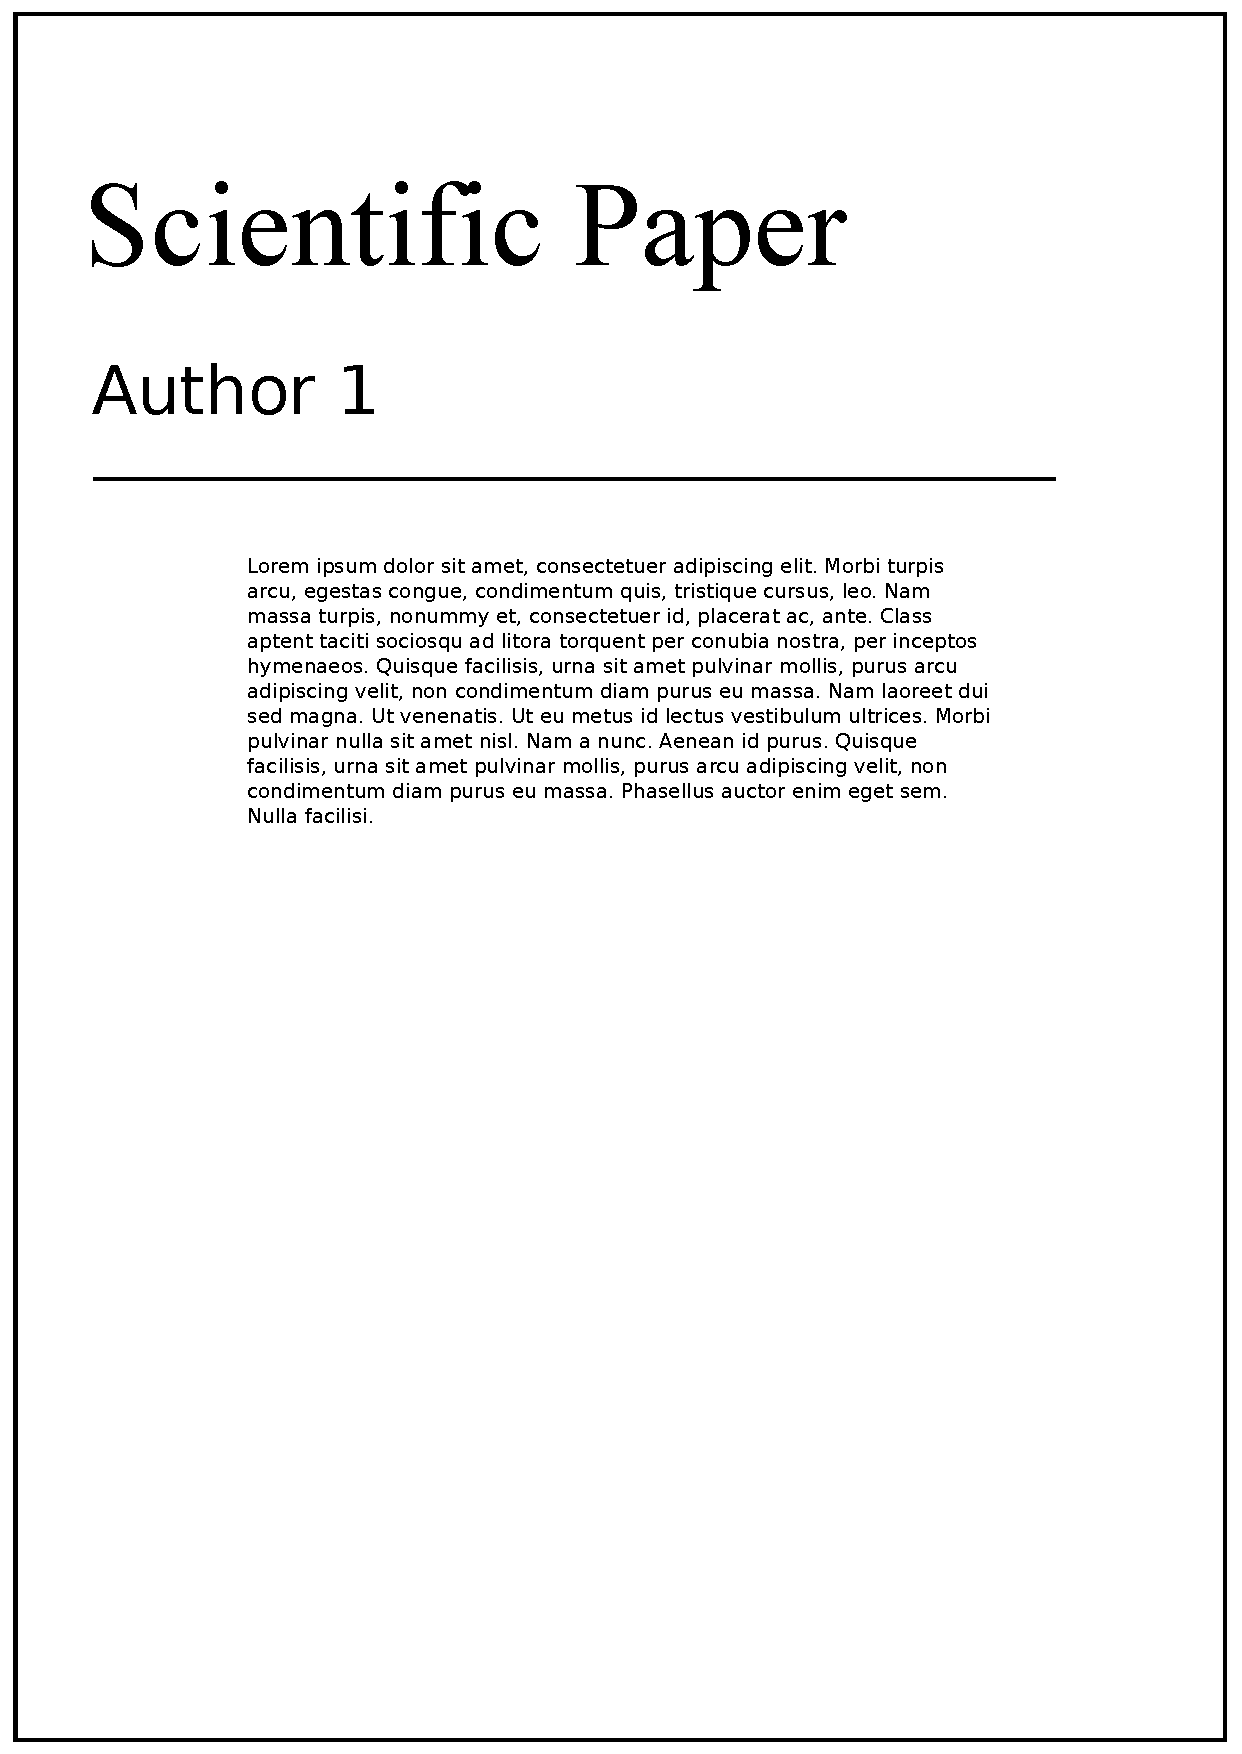
\includepdf[pages=-]{papers/paper1.pdf}

%****************************************************************
% Paper II
%****************************************************************
\chapter{Scientific Paper II}

\noindent List of authors\\

\noindent \textit{In \Proc \IntlConf \ldots} \textbf{IEEE}, 035303 (2017)
\cleardoublepage

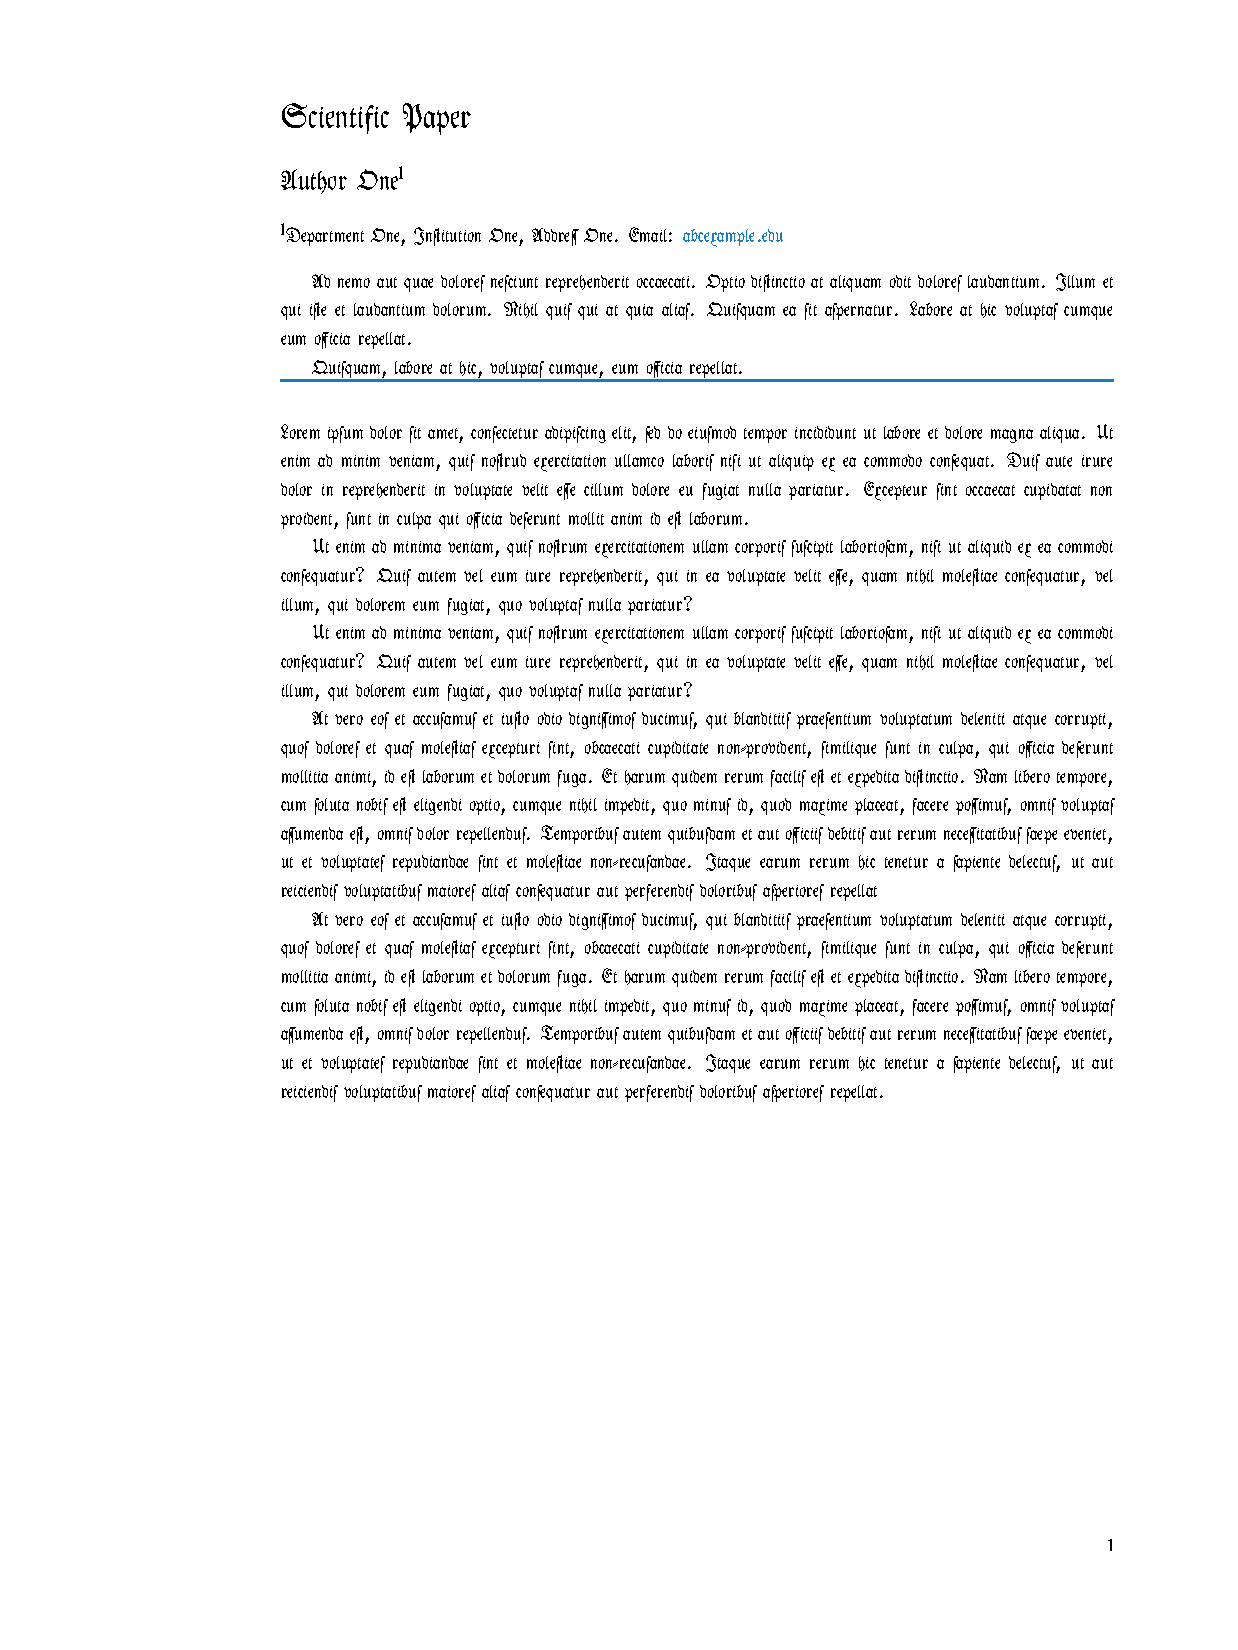
\includepdf[pages=-]{papers/paper2.pdf}



